\documentclass[12pt]{article}

\usepackage{titling}
\usepackage{blindtext}
\usepackage{fullpage}
\usepackage[round]{natbib}
\usepackage{multirow}
\usepackage{booktabs}
\usepackage{tabularx}
\usepackage{siunitx}
\usepackage{graphicx}
\usepackage{float}
\usepackage{hyperref}
\hypersetup{
    colorlinks,
    citecolor=blue,
    filecolor=black,
    linkcolor=red,
    urlcolor=blue
}
\newcommand{\colAwidth}{0.24\textwidth}
\newcommand{\colBwidth}{0.76\textwidth}

\newcommand{\colCwidth}{0.28\textwidth}
\newcommand{\colDwidth}{0.72\textwidth}

\newcommand{\colEwidth}{0.33\textwidth}
\newcommand{\colFwidth}{0.67\textwidth}

\newcounter{comnum} %Commonality Number
\newcommand{\cthecomnum}{C\thecomnum}
\newcommand{\cref}[1]{C\ref{#1}}

\newcounter{varnum} %Variability Number
\newcommand{\vthevarnum}{V\thevarnum}
\newcommand{\vref}[1]{V\ref{#1}}

\newcounter{parnum} %Parameter of Variation Number
\newcommand{\ptheparnum}{P\theparnum}
\newcommand{\pref}[1]{P\ref{#1}}

\newif\ifcomments\commentstrue

\ifcomments
\newcommand{\authornote}[3]{\textcolor{#1}{[#3 ---#2]}}
\newcommand{\todo}[1]{\textcolor{red}{[TODO: #1]}}
\else
\newcommand{\authornote}[3]{}
\newcommand{\todo}[1]{}
\fi

\newcommand{\wss}[1]{\authornote{blue}{SS}{#1}} %Spencer Smith
\newcommand{\jc}[1]{\authornote{red}{JC}{#1}} %Jacques Carette
\newcommand{\oo}[1]{\authornote{magenta}{OO}{#1}} %Olu Owojaiye
\newcommand{\pmi}[1]{\authornote{green}{PM}{#1}} %Peter Michalski
\newcommand{\ad}[1]{\authornote{cyan}{AD}{#1}} %Ao Dong

\begin{document}

\title{\bf{Commonality Analysis for Lattice Boltzmann Systems}} 
\author{Peter Michalski, \\Department of Computing and Software\\McMaster University}
\date{\today}

\begin{titlepage}
	\clearpage\maketitle
	\thispagestyle{empty}
	\begin{abstract}
		This report presents a commonality analysis for Lattice Boltzmann systems using a commonality analysis template based on \cite{SmithAndChen2004}. The document reviews both the methodology of commonality analysis and the details of Lattice Boltzmann systems. The commonality analysis itself consists of the following:
		\textit{i}) terminology and definitions; \textit{ii}) commonalities, or features that are common to all potential family members; \textit{iii}) variabilities, or features and characteristics that may vary among family members; and, \textit{iv}) parameters of variation, or the potential values that can be assigned to the variabilities. 
		The documentation of the above items for Lattice Boltzmann systems is clarified by decomposing each item into subsections on Lattice Boltzmann methods, input, output, nonfunctional requirements, and, where appropriate, system constraints.\\
		
		\noindent\textbf{Keywords:} Commonality analysis, Lattice Boltzmann methods, program family.
		
	\end{abstract}
\end{titlepage}

\pagenumbering{roman}

\newpage

\tableofcontents

\newpage

\pagenumbering{arabic}

\section{Introduction}
Lattice Boltzmann systems are well suited to development as a program family because they fit Parnas’s definition of a program family: “a set of programs whose common properties are so extensive that it is advantageous to study the common properties of the programs before analyzing individual members” \citep{parnas1976design}. Developing such systems as a program family is advantageous because Lattice Boltzmann systems share many common features, or commonalities. Furthermore, when there are differences between systems, the variabilities between them can be systematically considered. The purpose of this document is to record these commonalities and variabilities and show the relationships between them, and thus facilitate the specification and development of Lattice Boltzmann program family members. This document will be valuable in all future phases of system development and analysis. For instance, the requirements documentation for any Lattice Boltzmann systems will use the commonality analysis, since the requirements should refine the commonalities, which are shared requirements of all such systems. Moreover, the design of any future system will use this documentation to facilitate consideration of the variabilities, so that likely changes can be made to the system with a minimal amount of work.

The scope of the commonality analysis presented here can be considered both from the point of view of Lattice Boltzmann systems and from the point of view of software engineering methodologies. From the Lattice Boltzmann system perspective, the starting point for the current document is a commonality analysis. With respect to software engineering methodologies, the scope of the current report is restricted to informal methods, with the intention that the informal requirements will form a starting point for later development and refinement by formal methods.

The first section below provides an overview of the program family of Lattice Boltzmann systems, by reviewing what is involved in a commonality analysis and the basics of Lattice Boltzmann systems. After this, the basic terminology and definitions necessary for understanding the remainder of the document are provided. The definitions include terms used in describing a commonality analysis and terms that are used in defining the characteristics and properties of Lattice Boltzmann methods. The next three sections consist of the lists of commonalities, variabilities and parameters of variation, respectively. These three sections form the heart of the documentation and include an extensive set of cross-references to demonstrate the relationships between the different items. The final section provides information on unresolved issues.

\newpage
\section{Overview}
This section provides both an overview of the process of commonality analysis and of Lattice Boltzmann methods. The subsection on commonality analysis briefly introduces this topic, along with references that can be searched for further information. The subsection on Lattice Boltzmann methods outlines the basics of Lattice Boltzmann methods and of the scope of the commonality analysis.

\subsection{Commonality Analysis}
In some situations it is advantageous to develop a collection of related software products as a program family. The idea is that if the software products are similar enough, then it should be possible to predict what the products have in common, what differs between them and then reuse the common aspects and thus support rapid development of the family members. The idea of program families was introduced by \cite{dijkstra1972} and later investigated by \cite{parnas1976design,parnas1979designing}. More recently, \cite{weiss1997defining, weiss1998commonality, ardis1997defining} has considered the concept of a program family in the context of what he terms Family oriented Abstraction, Specification and Translation (FAST) \citep{cuka1997specifying,weiss1999software}.

In the approach advocated by Weiss, the first step is a commonality analysis. This analysis consists of systematically identifying and documenting the commonalities that all program family members share, the variabilities between family members and the terminology used in describing the family. A commonality analysis provides a systematic way of gaining confidence that a family is worth building and of deciding what the family members will be. A commonality analysis document provides the following benefits \cite{weiss1997defining, weiss1998commonality}:

\begin{enumerate}
	\item A starting point for the design of a domain specific languages (DSL): Once a DSL, or application modelling language, is developed the program family members can be rapidly generated by specifying a given family member using the language.
	\item A basis for a common design for all family members: When the software engineers come to designing the individual family members, they can take advantage of the commonalities to reuse code. Moreover, the variabilities can be considered in the design so that they can be easily accommodated. One approach to the design may be to decompose the system into components that can each be customized by specification of values for its various parameters, where the parameters correspond to the parameters of variation identified in the commonality analysis document.
	\item A historical reference: This document records the important issues concerning the scope and the nature of the family (as well as some unsolved issues) to facilitate the involvement of the participants in maintaining and evolving the family.
	\item A basis for re-engineering a domain: Existing projects may not have been developed using software engineering methodologies. The projects can be systematically reorganized and redesigned with the aid of a commonality analysis to unify the existing products.
	\item A basic training reference for new software developers: This document provides the necessary basic information for a new team-member to understand the family. 
\end{enumerate}

The next section will show that the above uses of the commonality analysis document will be beneficial for the development of a family of Lattice Boltzmann programs. The commonality analysis will benefit all subsequent stages in the software development process. For instance, as mentioned in the introduction, the commonalities will act as requirements that will be the starting point for writing a software requirements specification. The commonalities will be refined into specific requirements by fixing the value of their associated variabilities. The change in the values of the variabilities then corresponds to the change from one program family member to another.

As commonalities and variabilities are requirements, they should express “What” functionalities and qualities the system should have, and not mention “How” these requirements are to be accomplished. That is, the commonalities and variabilities should not involve design decisions. The design decisions will be made after the requirements for a family member have been specified. The one exception to this is system constraints, which are requirements that explicitly make design decisions. 

Besides the “What” versus “How” test, there are other tests that can be used to review commonalities and variabilities, as proposed by \cite{weiss1997defining}. One such test is the “what is ruled out” test. This test determines if a commonality or variability actually makes a decision because if no alternatives are ruled out then no decision has really been made. Another test is the “negation” test. If the negation of a decision represents a position that someone might argue for, then the original decision is likely to be meaningful. For instance, the statement that “the software should be reliable” has a negation that no one would likely argue for and thus the statement does not represent a good characterization of a goal for the system. 

In \cite{weiss1997defining} the stages of a commonality analysis are described in a systematic way. The stages include the following: prepare, plan, analyze, quantify and review. The stages are completed through the aid of a moderator and a series of meeting and preliminary documents and documentation reviews. The approach adopted here is to revise the original commonality analysis document produced by \cite{chen2003} and then make the new document available to others for review. The new document will be maintained in a concurrent versioning system repository so that multiple authors can work on it, and more importantly, so that the documentation’s revision history can be tracked and the documentation can be rolled back to an earlier version if necessary.

\subsection{Lattice Boltzmann Systems}
Lattice Boltzmann Methods (LBM) are a family of fluid dynamics algorithms for simulating single-phase and multiphase fluid flows, often incorporating additional physical complexities \citep{chen1998lattice}. They consider the behaviours of a collection of particles as a single unit at the mesoscopic scale. These methods predict the positional probability of a collection of particles moving through a lattice structure. Off the shelf (OTS) Lattice Boltzmann Solvers (LBS) allow for a range of fluid and physical model input parameters, computational parameters, and output parameters.

As LBS model fluid dynamics within a boundary using a predefined lattice structure, the methods rely on a two step calculation process. The first process is streaming, where the particles move along the lattice via links. The second process is collision, where energy and momentum is transferred among particles that collide \citep{bao2011lattice}.
There are many standardized lattice models - individual solvers within the family might only use a subset of them.
The LBM uses the initial parameters of the fluid to find the probability of where along the lattice linkages a group of particles are most likely to travel. It then moves the particles into the next node, and transfers the energy and momentum if a collision occurs. Then the process repeats for the duration of the modeling instance.\\


\begin{figure}[h!]
	\begin{center}
		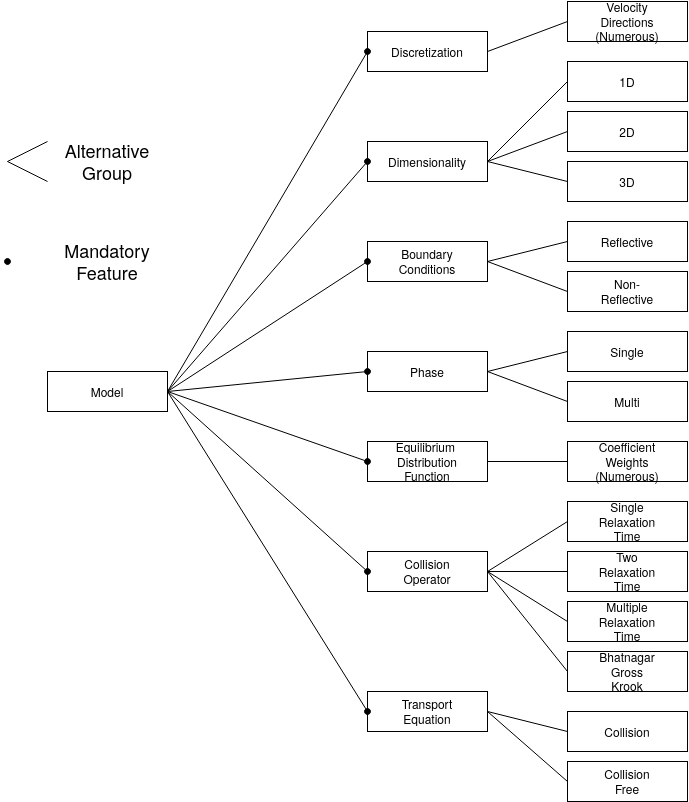
\includegraphics[width=0.5\textwidth]{FeatureDiagramLBS}
		\caption{LBS Model Feature Diagram}
		\label{LBSFeatureDiagram}
	\end{center}
\end{figure} 

\newpage
\section{Terminology and Definitions}
This section is divided into two subsections. The first discusses the terminology that comes from the software engineering field, while the second presents the definitions used in Lattice Boltzmann solvers. Common acronyms are also listed in this section. The lists are not intended to be read sequentially, but rather to be consulted for reference purposes; therefore, the terms are ordered alphabetically, with the consequence that some terms that appear early in the list depend on the definitions of later terms.

\subsection{Software Engineering Related Definitions and Acronyms}
\noindent\textbf{Commonality}: A requirement or goal common to all family members.\\

\noindent\textbf{Goal}: “Goals capture, at different levels of abstraction, the various objectives the system under consideration should achieve.” \cite{van2001goal}\\

\noindent\textbf{Program Family}: A set of programs that are analyzed and designed together starting from the initial stages of the software development life-cycle.\\

\noindent\textbf{Requirements}: A software requirement is: \textit{i}) a condition or capability needed by a user to solve a problem or achieve an objective; \textit{ii}) a condition or capability that must be met or possessed by a system or system component to satisfy a contract, standard, specification, or other formally imposed document; or, \textit{iii}) a documented representation of a condition or capability as in the above two definitions. \cite{thayer2000ieee}\\

\noindent\textbf{Variability}: A requirement or goal that varies between family members.

\subsection{Lattice Boltzmann Related Definitions and Acronyms}

\noindent\textbf{1D} 1-Dimensional\\

\noindent\textbf{2D}: 2-Dimensional\\

\noindent\textbf{3D}: 3-Dimensional\\

\noindent\textbf{BGK}: Bhatnagar-Gross-Krook\\

\noindent\textbf{CPU}: central processing unit\\

\noindent\textbf{GPU}: graphics processing unit\\

\noindent\textbf{MRT}: multi-relaxation-time\\

\noindent\textbf{SRT}: single-relaxation-time\\

\noindent\textbf{TRT}: two-relaxation-time\\
 
\noindent\textbf{LBM}: Lattice Boltzmann Methods\\

\noindent\textbf{LBS}: Lattice Boltzmann Solvers\\

\noindent\textbf{Velocity Directions}: The number of links connecting to each lattice node in the chosen model from neighbouring nodes. All nodes in a chosen lattice model will have the same number of links. A single link will connect between two adjacent nodes.
	

\newpage
\section{Commonalities}\label{comm_sec}

This section lists all the common features among all the potential family members. The commonalities are organized using the following abstraction of the system, which can be used to describe all Lattice Boltzmann systems: input information, then generate the simulation and finally output the results. Section \ref{comm_lbm} describes the commonalities for the simulation step. Section \ref{comm_in} highlights the input information that is required for all Lattice Boltzmann systems. The next section, Section \ref{comm_out}, shows the common features for the output of Lattice Boltzmann systems, such as the requirement that mesh information be written to files. (Although the output information could simply be written to the computer’s memory, in all practical applications it is desirable to have a persistent record of the output that was created.) The final section covers qualities of the system that cannot be classified as input, simulation generation or output. These commonalities are termed nonfunctional requirements of the system. For instance, all systems will have the goal that the response time to a user’s request is small enough to allow the user to focus on his/her problem and to maintain his/her train of thought, without being distracted by excessive waiting time. The commonality in this case is refined by a later variability because the specific requirement on the response time will depend on the intended usage of the mesh generating system. 

Each commonality below uses the same structure. All of the commonalities are assigned a unique item number, which takes the form of a natural number with the prefix ``C''. Following this, a description of the commonality is provided along with a list of related variabilities, which are given as hyperlinks that allow navigation of the document to the text describing the variability. Finally, each commonality ends with a summary of the history, including the date of creation and any dates of modification, along with a brief description of the modification. If necessary, a previous version of the document can be obtained by using the concurrent versioning system where the files are stored. 

\subsection{Lattice Boltzmann Method Solvers}\label{comm_lbm}
\noindent
\begin{minipage}{\textwidth}
	\renewcommand*{\arraystretch}{1.5}
	\begin{tabular}{| p{\colAwidth} | p{\colBwidth}|}
		\hline
		\bf Item Number& C\refstepcounter{comnum}\thecomnum{}\label{lattice} \\
		\hline
	\end{tabular}\\
	
	\begin{tabular}{| p{\colAwidth} | p{\colBwidth}|}		
		\hline
		\bf Description & A lattice discretizes a computational domain into a finite number of points. All LBS discretize the computational domain using a regular, evenly spaced grid within a boundary.\\
		\hline
		\bf Related Variability & \vref{numveldir} \vref{varcolop} \vref{varboundary}\\
		\hline
		\bf History & Created April 1, 2020 \\
		\hline
	\end{tabular}
\end{minipage}\\
~\newline\\
~\newline
\noindent
\begin{minipage}{\textwidth}
	\renewcommand*{\arraystretch}{1.5}
	\begin{tabular}{| p{\colAwidth} | p{\colBwidth}|}
		\hline
		\bf Item Number& C\refstepcounter{comnum}\thecomnum\label{collisionoperator} \\
		\hline
	\end{tabular}\\
	
	\begin{tabular}{| p{\colAwidth} | p{\colBwidth}|}		
		\hline
		\bf Description & All Lattice Boltzmann versions use a collision operator which concerns collisions between particles.\\
		\hline
		\bf Related Variability & \vref{dimensions} \vref{numveldir}\\
		\hline
		\bf History & Created April 1, 2020\\
		\hline
	\end{tabular}
\end{minipage}\\
~\newline\\
~\newline
\noindent
\begin{minipage}{\textwidth}
	\renewcommand*{\arraystretch}{1.5}
	\begin{tabular}{| p{\colAwidth} | p{\colBwidth}|}
		\hline
		\bf Item Number& C\refstepcounter{comnum}\thecomnum\label{probabilitydensityfunc} \\
		\hline
	\end{tabular}\\
	
	\begin{tabular}{| p{\colAwidth} | p{\colBwidth}|}		
		\hline
		\bf Description & All Lattice Boltzmann versions user a probability density function to give the probability that fluid has moved into a specific domain.\\
		\hline
		\bf Related Variability & \vref{dimensions}\\
		\hline
		\bf History & Created April 1, 2020\\
		\hline
	\end{tabular}
\end{minipage}\\
\begin{minipage}{\textwidth}
	\renewcommand*{\arraystretch}{1.5}
	\begin{tabular}{| p{\colAwidth} | p{\colBwidth}|}
		\hline
		\bf Item Number& C\refstepcounter{comnum}\thecomnum\label{equildistfunc} \\
		\hline
	\end{tabular}\\
	
	\begin{tabular}{| p{\colAwidth} | p{\colBwidth}|}		
		\hline
		\bf Description & Every Lattice Boltzmann version uses an equilibrium distribution function to capture the probability distribution of particles.\\
		\hline
		\bf Related Variability & \vref{varedf} \vref{edfstorage} \vref{edfcoeff}\\
		\hline
		\bf History & Created April 1, 2020\\
		\hline
	\end{tabular}
\end{minipage}\\
~\newline\\
~\newline
\noindent
\begin{minipage}{\textwidth}
	\renewcommand*{\arraystretch}{1.5}
	\begin{tabular}{| p{\colAwidth} | p{\colBwidth}|}
		\hline
		\bf Item Number& C\refstepcounter{comnum}\thecomnum\label{Boltzmanntransequ} \\
		\hline
	\end{tabular}\\
	
	\begin{tabular}{| p{\colAwidth} | p{\colBwidth}|}		
		\hline
		\bf Description & Every Lattice Boltzmann version uses a Boltzmann transport equation to describe the statistical behaviour of a system that does not have collisions.\\
		\hline
		\bf Related Variability & \vref{vartraneq}\\
		\hline
		\bf History & Created April 1, 2020\\
		\hline
	\end{tabular}
\end{minipage}\\
\subsection{Input}\label{comm_in}
\noindent
\begin{minipage}{\textwidth}
	\renewcommand*{\arraystretch}{1.5}
	\begin{tabular}{| p{\colAwidth} | p{\colBwidth}|}
		\hline
		\bf Item Number& C\refstepcounter{comnum}\thecomnum\label{fluidandboundaryinfo} \\
		\hline
	\end{tabular}\\
	
	\begin{tabular}{| p{\colAwidth} | p{\colBwidth}|}		
		\hline
		\bf Description & The LBS require fluid, model, and boundary information for the problem.\\
		\hline
		\bf Related Variability & \vref{interface}\\
		\hline
		\bf History & Created April 1, 2020\\
		\hline
	\end{tabular}
\end{minipage}\\
\subsection{Output}\label{comm_out}
\noindent
\begin{minipage}{\textwidth}
	\renewcommand*{\arraystretch}{1.5}
	\begin{tabular}{| p{\colAwidth} | p{\colBwidth}|}
		\hline
		\bf Item Number& C\refstepcounter{comnum}\thecomnum\label{predictionstomemory} \\
		\hline
	\end{tabular}\\
	
	\begin{tabular}{| p{\colAwidth} | p{\colBwidth}|}		
		\hline
		\bf Description & LBS write fluid parameter predictions to memory.\\
		\hline
		\bf Related Variability & \vref{varvisual} \vref{formatoutput} \\
		\hline
		\bf History & Created April 1, 2020\\
		\hline
	\end{tabular}
\end{minipage}\\
\subsection{Nonfunctional Requirements}\label{comm_nfr}
\noindent
\begin{minipage}{\textwidth}
	\renewcommand*{\arraystretch}{1.5}
	\begin{tabular}{| p{\colAwidth} | p{\colBwidth}|}
		\hline
		\bf Item Number& C\refstepcounter{comnum}\thecomnum\label{precision} \\
		\hline
	\end{tabular}\\
	
	\begin{tabular}{| p{\colAwidth} | p{\colBwidth}|}		
		\hline
		\bf Description & LBS provides the precision required for the particular problems it is intended to solve.\\
		\hline
		\bf Related Variability & \vref{varprecise}\\
		\hline
		\bf History & Created April 1, 2020\\
		\hline
	\end{tabular}
\end{minipage}\\
~\newline\\
~\newline

\noindent
\begin{minipage}{\textwidth}
	\renewcommand*{\arraystretch}{1.5}
	\begin{tabular}{| p{\colAwidth} | p{\colBwidth}|}
		\hline
		\bf Item Number& C\refstepcounter{comnum}\thecomnum\label{accuracy} \\
		\hline
	\end{tabular}\\
	
	\begin{tabular}{| p{\colAwidth} | p{\colBwidth}|}		
		\hline
		\bf Description & LBS provides the accuracy required for the particular problems it is intended to solve.\\
		\hline
		\bf Related Variability & \vref{varaccuracy}\\
		\hline
		\bf History & Created April 1, 2020\\
		\hline
	\end{tabular}
\end{minipage}\\
~\newline\\
~\newline

\noindent
\begin{minipage}{\textwidth}
	\renewcommand*{\arraystretch}{1.5}
	\begin{tabular}{| p{\colAwidth} | p{\colBwidth}|}
		\hline
		\bf Item Number& C\refstepcounter{comnum}\thecomnum\label{performance} \\
		\hline
	\end{tabular}\\
	
	\begin{tabular}{| p{\colAwidth} | p{\colBwidth}|}		
		\hline
		\bf Description & The response time is small enough to allow the user to focus on their problem without being distracted by excessive waiting times.\\
		\hline
		\bf Related Variability & \vref{varresponsetime}\\
		\hline
		\bf History & Created April 1, 2020\\
		\hline
	\end{tabular}
\end{minipage}\\
~\newline\\
~\newline

\noindent
\begin{minipage}{\textwidth}
	\renewcommand*{\arraystretch}{1.5}
	\begin{tabular}{| p{\colAwidth} | p{\colBwidth}|}
		\hline
		\bf Item Number& C\refstepcounter{comnum}\thecomnum\label{portability} \\
		\hline
	\end{tabular}\\
	
	\begin{tabular}{| p{\colAwidth} | p{\colBwidth}|}		
		\hline
		\bf Description & LBS will be as portable to other operating systems as required by the users.\\
		\hline
		\bf Related Variability & \vref{varportability}\\
		\hline
		\bf History & Created April 1, 2020\\
		\hline
	\end{tabular}
\end{minipage}\\
~\newline\\
~\newline

\noindent
\begin{minipage}{\textwidth}
	\renewcommand*{\arraystretch}{1.5}
	\begin{tabular}{| p{\colAwidth} | p{\colBwidth}|}
		\hline
		\bf Item Number& C\refstepcounter{comnum}\thecomnum\label{usability} \\
		\hline
	\end{tabular}\\
	
	\begin{tabular}{| p{\colAwidth} | p{\colBwidth}|}		
		\hline
		\bf Description & The use of LBS is easy and efficient.\\
		\hline
		\bf Related Variability & \vref{varusability}\\
		\hline
		\bf History & Created April 1, 2020\\
		\hline
	\end{tabular}
\end{minipage}\\
\newpage
\section{Variabilities}\label{var_sec}
This section provides a list of characteristics that may vary among family members. As in Section \ref{comm_sec}, the first three subsections on variabilities are organized into the following sublists: Mesh Generation, Input and Output. The final two subsections list variabilities that can be characterized as system constraints and as nonfunctional requirements. 

As for the commonalities, each variability is labelled with a unique item number. In this case the numbers are prepended with the letter ``V''. The other four headings provided for each variability are: Description, Related Commonality, Related Parameter and History. The related commonalities and parameters are given as a set of identifiers that respectively refer back to the previous section on commonalities or refer forward to the next section on parameters of variation.

\subsection{Lattice Boltzmann Method Solvers}
\noindent
\begin{minipage}{\textwidth}
	\renewcommand*{\arraystretch}{1.5}
	\begin{tabular}{| p{\colCwidth} | p{\colDwidth}|}
		\hline
		\bf Item Number& V\refstepcounter{varnum}\thevarnum\label{parallel} \\
		\hline
	\end{tabular}\\
	
	\begin{tabular}{| p{\colCwidth} | p{\colDwidth}|}		
		\hline
		\bf Description & LBS may use a framework for parallel processing of the model.\\
		\hline
		\bf Related Commonality & None\\
		\hline
		\bf Related Parameter & \pref{parparallel}\\
		\hline
		\bf History & Created April 1, 2020\\
		\hline
	\end{tabular}
\end{minipage}\\
~\newline\\
\begin{minipage}{\textwidth}
	\renewcommand*{\arraystretch}{1.5}
	\begin{tabular}{| p{\colCwidth} | p{\colDwidth}|}
		\hline
		\bf Item Number& V\refstepcounter{varnum}\thevarnum\label{varedf} \\
		\hline
	\end{tabular}\\
	
	\begin{tabular}{| p{\colCwidth} | p{\colDwidth}|}		
		\hline
		\bf Description & Different versions of an equilibrium distribution function can capture the probability distribution of particles.\\
		\hline
		\bf Related Commonality & \cref{equildistfunc}\\
		\hline
		\bf Related Parameter & \pref{paredf}\\
		\hline
		\bf History & Created April 1, 2020\\
		\hline
	\end{tabular}
\end{minipage}\\
~\newline\\
~\newline
\noindent
\begin{minipage}{\textwidth}
	\renewcommand*{\arraystretch}{1.5}
	\begin{tabular}{| p{\colCwidth} | p{\colDwidth}|}
		\hline
		\bf Item Number& V\refstepcounter{varnum}\thevarnum\label{edfstorage} \\
		\hline
	\end{tabular}\\
	
	\begin{tabular}{| p{\colCwidth} | p{\colDwidth}|}		
		\hline
		\bf Description & Storage patters for distribution function can vary.\\
		\hline
		\bf Related Commonality & \cref{equildistfunc}\\
		\hline
		\bf Related Parameter & \pref{parstorage}\\
		\hline
		\bf History & Created April 1, 2020\\
		\hline
	\end{tabular}
\end{minipage}\\
~\newline\\
~\newline
\noindent
\begin{minipage}{\textwidth}
	\renewcommand*{\arraystretch}{1.5}
	\begin{tabular}{| p{\colCwidth} | p{\colDwidth}|}
		\hline
		\bf Item Number& V\refstepcounter{varnum}\thevarnum\label{edfcoeff} \\
		\hline
	\end{tabular}\\
	
	\begin{tabular}{| p{\colCwidth} | p{\colDwidth}|}		
		\hline
		\bf Description & Coefficients for distribution function can vary.\\
		\hline
		\bf Related Commonality & \cref{equildistfunc}\\
		\hline
		\bf Related Parameter & \pref{paredfcoeff}\\
		\hline
		\bf History & Created April 1, 2020\\
		\hline
	\end{tabular}
\end{minipage}\\
~\newline\\
~\newline
\noindent
\begin{minipage}{\textwidth}
	\renewcommand*{\arraystretch}{1.5}
	\begin{tabular}{| p{\colCwidth} | p{\colDwidth}|}
		\hline
		\bf Item Number& V\refstepcounter{varnum}\thevarnum\label{dimensions} \\
		\hline
	\end{tabular}\\
	
	\begin{tabular}{| p{\colCwidth} | p{\colDwidth}|}		
		\hline
		\bf Description & The number of dimensions in the lattice of the model can vary.\\
		\hline
		\bf Related Commonality & \cref{lattice} \cref{probabilitydensityfunc}\\
		\hline
		\bf Related Parameter & \pref{pardimensions}\\
		\hline
		\bf History & Created April 1, 2020\\
		\hline
	\end{tabular}
\end{minipage}\\
~\newline\\
~\newline
\noindent
\begin{minipage}{\textwidth}
	\renewcommand*{\arraystretch}{1.5}
	\begin{tabular}{| p{\colCwidth} | p{\colDwidth}|}
		\hline
		\bf Item Number& V\refstepcounter{varnum}\thevarnum\label{numveldir} \\
		\hline
	\end{tabular}\\
	
	\begin{tabular}{| p{\colCwidth} | p{\colDwidth}|}		
		\hline 
		\bf Description & The number of velocity directions in the lattice of the model can vary.\\
		\hline
		\bf Related Commonality & \cref{lattice} \cref{collisionoperator}\\
		\hline
		\bf Related Parameter & \pref{parveldir}\\
		\hline
		\bf History & Created April 1, 2020\\
		\hline
	\end{tabular}
\end{minipage}\\
~\newline\\
~\newline
\noindent
\begin{minipage}{\textwidth}
	\renewcommand*{\arraystretch}{1.5}
	\begin{tabular}{| p{\colCwidth} | p{\colDwidth}|}
		\hline
		\bf Item Number& V\refstepcounter{varnum}\thevarnum\label{varcolop} \\
		\hline
	\end{tabular}\\
	
	\begin{tabular}{| p{\colCwidth} | p{\colDwidth}|}		
		\hline
		\bf Description & Various collision operators can be used.\\
		\hline
		\bf Related Commonality & \cref{lattice} \cref{collisionoperator}\\
		\hline
		\bf Related Parameter & \pref{parcollisop}\\
		\hline
		\bf History & Created April 1, 2020\\
		\hline
	\end{tabular}
\end{minipage}\\
~\newline\\
~\newline
\noindent
\begin{minipage}{\textwidth}
	\renewcommand*{\arraystretch}{1.5}
	\begin{tabular}{| p{\colCwidth} | p{\colDwidth}|}
		\hline
		\bf Item Number& V\refstepcounter{varnum}\thevarnum\label{vartraneq} \\
		\hline
	\end{tabular}\\
	
	\begin{tabular}{| p{\colCwidth} | p{\colDwidth}|}		
		\hline
		\bf Description & Various transport equations can be used to describe the statistical behaviour of the system\\
		\hline
		\bf Related Commonality & \cref{Boltzmanntransequ}\\
		\hline
		\bf Related Parameter & \pref{partransequ}\\
		\hline
		\bf History & Created April 1, 2020\\
		\hline
	\end{tabular}
\end{minipage}\\
~\newline\\
~\newline
\noindent
\begin{minipage}{\textwidth}
	\renewcommand*{\arraystretch}{1.5}
	\begin{tabular}{| p{\colCwidth} | p{\colDwidth}|}
		\hline
		\bf Item Number&  V\refstepcounter{varnum}\thevarnum\label{numberoffluids} \\
		\hline
	\end{tabular}\\
	
	\begin{tabular}{| p{\colCwidth} | p{\colDwidth}|}		
		\hline
		\bf Description & The number of fluids allowed in the LBS.\\
		\hline
		\bf Related Commonality & \cref{fluidandboundaryinfo}\\
		\hline
		\bf Related Parameter & \pref{parfluids}\\
		\hline
		\bf History & Created April 1, 2020\\
		\hline
	\end{tabular}
\end{minipage}\\
~\newline\\
~\newline
\noindent
\begin{minipage}{\textwidth}
	\renewcommand*{\arraystretch}{1.5}
	\begin{tabular}{| p{\colCwidth} | p{\colDwidth}|}
		\hline
		\bf Item Number&  V\refstepcounter{varnum}\thevarnum\label{typefluidparm} \\
		\hline
	\end{tabular}\\
	
	\begin{tabular}{| p{\colCwidth} | p{\colDwidth}|}		
		\hline
		\bf Description & The type of fluid parameters.\\
		\hline
		\bf Related Commonality & \cref{fluidandboundaryinfo}\\
		\hline
		\bf Related Parameter & \pref{partypeparm}\\
		\hline
		\bf History & Created April 1, 2020\\
		\hline
	\end{tabular}
\end{minipage}\\
~\newline\\
~\newline
\noindent
\begin{minipage}{\textwidth}
	\renewcommand*{\arraystretch}{1.5}
	\begin{tabular}{| p{\colCwidth} | p{\colDwidth}|}
		\hline
		\bf Item Number&  V\refstepcounter{varnum}\thevarnum\label{varboundary} \\
		\hline
	\end{tabular}\\
	
	\begin{tabular}{| p{\colCwidth} | p{\colDwidth}|}		
		\hline
		\bf Description & The boundary of the lattice can have varied conditions.\\
		\hline
		\bf Related Commonality & \cref{lattice}\\
		\hline
		\bf Related Parameter & \pref{parboundary}\\
		\hline
		\bf History & Created April 1, 2020\\
		\hline
	\end{tabular}
\end{minipage}\\
\subsection{Input}
\noindent
\begin{minipage}{\textwidth}
	\renewcommand*{\arraystretch}{1.5}
	\begin{tabular}{| p{\colCwidth} | p{\colDwidth}|}
		\hline
		\bf Item Number& V\refstepcounter{varnum}\thevarnum\label{interface} \\
		\hline
	\end{tabular}\\
	
	\begin{tabular}{| p{\colCwidth} | p{\colDwidth}|}		
		\hline
		\bf Description & The input interface can vary between LBS.\\
		\hline
		\bf Related Commonality & \cref{fluidandboundaryinfo}\\
		\hline
		\bf Related Parameter & \pref{parinterface}\\
		\hline
		\bf History & Created April 1, 2020\\
		\hline
	\end{tabular}
\end{minipage}\\
\subsection{Output}
\noindent
\begin{minipage}{\textwidth}
	\renewcommand*{\arraystretch}{1.5}
	\begin{tabular}{| p{\colCwidth} | p{\colDwidth}|}
		\hline
		\bf Item Number& V\refstepcounter{varnum}\thevarnum\label{varvisual} \\
		\hline
	\end{tabular}\\
	
	\begin{tabular}{| p{\colCwidth} | p{\colDwidth}|}		
		\hline
		\bf Description & Visual presentation of the prediction.\\
		\hline
		\bf Related Commonality & \cref{predictionstomemory}\\
		\hline
		\bf Related Parameter & \pref{parvarvisual}\\
		\hline
		\bf History & Created April 1, 2020\\
		\hline
	\end{tabular}
\end{minipage}\\
~\newline\\
~\newline
\noindent
\begin{minipage}{\textwidth}
	\renewcommand*{\arraystretch}{1.5}
	\begin{tabular}{| p{\colCwidth} | p{\colDwidth}|}
		\hline
		\bf Item Number& V\refstepcounter{varnum}\thevarnum\label{formatoutput} \\
		\hline
	\end{tabular}\\
	
	\begin{tabular}{| p{\colCwidth} | p{\colDwidth}|}		
		\hline
		\bf Description & Format of prediction information.\\
		\hline
		\bf Related Commonality & \cref{predictionstomemory}\\
		\hline
		\bf Related Parameter & \pref{parformatoutput}\\
		\hline
		\bf History & Created April 1, 2020\\
		\hline
	\end{tabular}
\end{minipage}\\
\subsection{System Constraints}
\noindent
\begin{minipage}{\textwidth}
	\renewcommand*{\arraystretch}{1.5}
	\begin{tabular}{| p{\colCwidth} | p{\colDwidth}|}
		\hline
		\bf Item Number& V\refstepcounter{varnum}\thevarnum\label{processing} \\
		\hline
	\end{tabular}\\
	
	\begin{tabular}{| p{\colCwidth} | p{\colDwidth}|}		
		\hline
		\bf Description & Hardware which processes the calculations\\
		\hline
		\bf Related Commonality & None \\
		\hline
		\bf Related Parameter & \pref{parprocessing}\\
		\hline
		\bf History & Created April 1, 2020\\
		\hline
	\end{tabular}
\end{minipage}\\
~\newline\\
~\newline
\noindent
\begin{minipage}{\textwidth}
	\renewcommand*{\arraystretch}{1.5}
	\begin{tabular}{| p{\colCwidth} | p{\colDwidth}|}
		\hline
		\bf Item Number& V\refstepcounter{varnum}\thevarnum\label{operatingsystem} \\
		\hline
	\end{tabular}\\
	
	\begin{tabular}{| p{\colCwidth} | p{\colDwidth}|}		
		\hline
		\bf Description & Operating systems on which LBS runs.\\
		\hline
		\bf Related Commonality & None \\
		\hline
		\bf Related Parameter & \pref{paropsystem}\\
		\hline
		\bf History & Created April 1, 2020\\
		\hline
	\end{tabular}
\end{minipage}\\
~\newline\\
~\newline
\noindent
\begin{minipage}{\textwidth}
	\renewcommand*{\arraystretch}{1.5}
	\begin{tabular}{| p{\colCwidth} | p{\colDwidth}|}
		\hline
		\bf Item Number& V\refstepcounter{varnum}\thevarnum\label{storage} \\
		\hline
	\end{tabular}\\
	
	\begin{tabular}{| p{\colCwidth} | p{\colDwidth}|}		
		\hline
		\bf Description & Amount of storage and memory needed for the LBS.\\
		\hline
		\bf Related Commonality & None \\
		\hline
		\bf Related Parameter & \pref{parstorageconst}\\
		\hline
		\bf History & Created April 1, 2020\\
		\hline
	\end{tabular}
\end{minipage}\\
\subsection{Nonfunctional Requirements}
\noindent
\begin{minipage}{\textwidth}
	\renewcommand*{\arraystretch}{1.5}
	\begin{tabular}{| p{\colCwidth} | p{\colDwidth}|}
		\hline
		\bf Item Number& V\refstepcounter{varnum}\thevarnum\label{varprecise} \\
		\hline
	\end{tabular}\\
	
	\begin{tabular}{| p{\colCwidth} | p{\colDwidth}|}		
		\hline
		\bf Description & The precision needed for each input and output.\\
		\hline
		\bf Related Commonality & \cref{precision}\\
		\hline
		\bf Related Parameter & \pref{parprecise}\\
		\hline
		\bf History & Created April 1, 2020\\
		\hline
	\end{tabular}
\end{minipage}\\
~\newline\\
~\newline
\noindent
\begin{minipage}{\textwidth}
	\renewcommand*{\arraystretch}{1.5}
	\begin{tabular}{| p{\colCwidth} | p{\colDwidth}|}
		\hline
		\bf Item Number& V\refstepcounter{varnum}\thevarnum\label{varaccuracy} \\
		\hline
	\end{tabular}\\
	
	\begin{tabular}{| p{\colCwidth} | p{\colDwidth}|}		
		\hline
		\bf Description & The required accuracy for the output.\\
		\hline
		\bf Related Commonality & \cref{accuracy}\\
		\hline
		\bf Related Parameter & \pref{paraccuracy}\\
		\hline
		\bf History & Created April 1, 2020\\
		\hline
	\end{tabular}
\end{minipage}\\
~\newline\\
~\newline
\noindent
\begin{minipage}{\textwidth}
	\renewcommand*{\arraystretch}{1.5}
	\begin{tabular}{| p{\colCwidth} | p{\colDwidth}|}
		\hline
		\bf Item Number& V\refstepcounter{varnum}\thevarnum\label{varresponsetime} \\
		\hline
	\end{tabular}\\
	
	\begin{tabular}{| p{\colCwidth} | p{\colDwidth}|}		
		\hline
		\bf Description & The response time required for user interaction with the system varies.\\
		\hline
		\bf Related Commonality & \cref{performance}\\
		\hline
		\bf Related Parameter & \pref{parresponse}\\
		\hline
		\bf History & Created April 1, 2020\\
		\hline
	\end{tabular}
\end{minipage}\\
~\newline\\
~\newline
\noindent
\begin{minipage}{\textwidth}
	\renewcommand*{\arraystretch}{1.5}
	\begin{tabular}{| p{\colCwidth} | p{\colDwidth}|}
		\hline
		\bf Item Number& V\refstepcounter{varnum}\thevarnum\label{varportability} \\
		\hline
	\end{tabular}\\
	
	\begin{tabular}{| p{\colCwidth} | p{\colDwidth}|}		
		\hline
		\bf Description & The operating systems on which a LBS can run.\\
		\hline
		\bf Related Commonality & \cref{portability}\\
		\hline
		\bf Related Parameter & \pref{parportability}\\
		\hline
		\bf History & Created April 1, 2020\\
		\hline
	\end{tabular}
\end{minipage}\\
~\newline\\
~\newline
\noindent
\begin{minipage}{\textwidth}
	\renewcommand*{\arraystretch}{1.5}
	\begin{tabular}{| p{\colCwidth} | p{\colDwidth}|}
		\hline
		\bf Item Number& V\refstepcounter{varnum}\thevarnum\label{varusability} \\
		\hline
	\end{tabular}\\
	
	\begin{tabular}{| p{\colCwidth} | p{\colDwidth}|}		
		\hline
		\bf Description & The ease with which LBS can effectively be run varies.\\
		\hline
		\bf Related Commonality & \cref{usability}\\
		\hline
		\bf Related Parameter & \pref{parusability}\\
		\hline
		\bf History & Created April 1, 2020\\
		\hline
	\end{tabular}
\end{minipage}\\
\newpage
\section{Parameters of Variation}
This section specifies the parameters of variation for the variabilities listed in Section \ref{var_sec}. They are organized into the same five subcategories as employed previously: Mesh Generation, Input, Output, System Constraints, Nonfunctional Requirements. 

Each parameter of variation is given a unique identifier of the form “P” followed by a natural number. The corresponding variability is listed and a hyperlink is provided that allows navigation back to the appropriate item in Section \ref{var_sec}. The final entry for each parameter of variation is the binding time, which is the time in the software lifecycle when the variability is fixed. The binding time could be during specification, or during building
of the system (compile time), or during execution of the system (run time). It is possible to have a mixture of binding times. For instance, a parameter of variation could have a binding time of “specification or building” to represent that the parameter could be set at specification time, or it could be postponed until the given family member is built. The choice of postponing the decision until the build would be associated with the presence of a domain specific language that would allow postponing decisions on the values of the parameter of variation.

\subsection{Lattice Boltzmann Method Solvers}
\noindent
\begin{minipage}{\textwidth}
	\renewcommand*{\arraystretch}{1.5}
	\begin{tabular}{| p{\colEwidth} | p{\colFwidth}|}
		\hline
		\bf Item Number& P\refstepcounter{parnum}\theparnum\label{parparallel} \\
		\hline
	\end{tabular}\\
	
	\begin{tabular}{| p{\colEwidth} | p{\colFwidth}|}		
		\hline
		\bf Corresponding Variability & \vref{parallel}\\
		\hline
		\bf Range of Parameters & OpenMP, OpenCL, CUDA, or MPI are used if LBS is parallel.\\
		\hline
		\bf Binding Time & Build Time\\
		\hline
	\end{tabular}
\end{minipage}\\
~\newline\\
~\newline
\noindent
\begin{minipage}{\textwidth}
	\renewcommand*{\arraystretch}{1.5}
	\begin{tabular}{| p{\colEwidth} | p{\colFwidth}|}
		\hline
		\bf Item Number& P\refstepcounter{parnum}\theparnum\label{paredf} \\
		\hline
	\end{tabular}\\
	
	\begin{tabular}{| p{\colEwidth} | p{\colFwidth}|}		
		\hline
		\bf Corresponding Variability & \vref{parallel}\\
		\hline
		\bf Range of Parameters & Equilibrium can be approximated up to different orders in incompressible or compressible versions.\\
		\hline
		\bf Binding Time & Build Time\\
		\hline
	\end{tabular}
\end{minipage}\\
~\newline\\
~\newline
\noindent
\begin{minipage}{\textwidth}
	\renewcommand*{\arraystretch}{1.5}
	\begin{tabular}{| p{\colEwidth} | p{\colFwidth}|}
		\hline
		\bf Item Number& P\refstepcounter{parnum}\theparnum\label{parstorage} \\
		\hline
	\end{tabular}\\
	
	\begin{tabular}{| p{\colEwidth} | p{\colFwidth}|}		
		\hline
		\bf Corresponding Variability & \vref{edfstorage}\\
		\hline
		\bf Range of Parameters & Single and multiple array storage patterns can be used.\\
		\hline
		\bf Binding Time & Build Time\\
		\hline
	\end{tabular}
\end{minipage}\\
~\newline\\
~\newline
\noindent
\begin{minipage}{\textwidth}
	\renewcommand*{\arraystretch}{1.5}
	\begin{tabular}{| p{\colEwidth} | p{\colFwidth}|}
		\hline
		\bf Item Number& P\refstepcounter{parnum}\theparnum\label{paredfcoeff} \\
		\hline
	\end{tabular}\\
	
	\begin{tabular}{| p{\colEwidth} | p{\colFwidth}|}		
		\hline
		\bf Corresponding Variability & \vref{edfcoeff}\\
		\hline
		\bf Range of Parameters & Numerous coefficients for equilibrium distribution function based on number of velocity directions. \\
		\hline
		\bf Binding Time & Build Time\\
		\hline
	\end{tabular}
\end{minipage}\\
~\newline\\
~\newline
\noindent
\begin{minipage}{\textwidth}
	\renewcommand*{\arraystretch}{1.5}
	\begin{tabular}{| p{\colEwidth} | p{\colFwidth}|}
		\hline
		\bf Item Number& P\refstepcounter{parnum}\theparnum\label{pardimensions} \\
		\hline
	\end{tabular}\\
	
	\begin{tabular}{| p{\colEwidth} | p{\colFwidth}|}		
		\hline
		\bf Corresponding Variability & \vref{dimensions}\\
		\hline
		\bf Range of Parameters & LBS models can have up to 3 dimensions.\\
		\hline
		\bf Binding Time & Build Time or Run Time\\
		\hline
	\end{tabular}
\end{minipage}\\
~\newline\\
~\newline
\noindent
\begin{minipage}{\textwidth}
	\renewcommand*{\arraystretch}{1.5}
	\begin{tabular}{| p{\colEwidth} | p{\colFwidth}|}
		\hline
		\bf Item Number& P\refstepcounter{parnum}\theparnum\label{parveldir} \\
		\hline
	\end{tabular}\\
	
	\begin{tabular}{| p{\colEwidth} | p{\colFwidth}|}		
		\hline
		\bf Corresponding Variability & \vref{numveldir}\\
		\hline
		\bf Range of Parameters & One dimensional models include options of 2, 3, and 5 velocity directions. Two dimensional models include options of 9, 13, and 15 velocity directions. Three dimensional models include options of 15, 19, and 27 velocity directions. \\
		\hline
		\bf Binding Time & Build Time or Run Time\\
		\hline
	\end{tabular}
\end{minipage}\\
~\newline\\
~\newline
\noindent
\begin{minipage}{\textwidth}
	\renewcommand*{\arraystretch}{1.5}
	\begin{tabular}{| p{\colEwidth} | p{\colFwidth}|}
		\hline
		\bf Item Number& P\refstepcounter{parnum}\theparnum\label{parcollisop} \\
		\hline
	\end{tabular}\\
	
	\begin{tabular}{| p{\colEwidth} | p{\colFwidth}|}		
		\hline
		\bf Corresponding Variability & \vref{varcolop}\\
		\hline
		\bf Range of Parameters & SRT, TRT, MRT, BGK collision operators.\\
		\hline
		\bf Binding Time & Build Time\\
		\hline
	\end{tabular}
\end{minipage}\\
~\newline\\
~\newline
\noindent
\begin{minipage}{\textwidth}
	\renewcommand*{\arraystretch}{1.5}
	\begin{tabular}{| p{\colEwidth} | p{\colFwidth}|}
		\hline
		\bf Item Number& P\refstepcounter{parnum}\theparnum\label{partransequ} \\
		\hline
	\end{tabular}\\
	
	\begin{tabular}{| p{\colEwidth} | p{\colFwidth}|}		
		\hline
		\bf Corresponding Variability & \vref{vartraneq}\\
		\hline
		\bf Range of Parameters & Collision and collision free transport equations.\\
		\hline
		\bf Binding Time & Build Time\\
		\hline
	\end{tabular}
\end{minipage}\\
~\newline\\
~\newline
\noindent
\begin{minipage}{\textwidth}
	\renewcommand*{\arraystretch}{1.5}
	\begin{tabular}{| p{\colEwidth} | p{\colFwidth}|}
		\hline
		\bf Item Number& P\refstepcounter{parnum}\theparnum\label{parfluids} \\
		\hline
	\end{tabular}\\
	
	\begin{tabular}{| p{\colEwidth} | p{\colFwidth}|}		
		\hline
		\bf Corresponding Variability & \vref{numberoffluids}\\
		\hline
		\bf Range of Parameters & LBS can model one or more fluids.\\
		\hline
		\bf Binding Time & Build Time\\
		\hline
	\end{tabular}
\end{minipage}\\
~\newline\\
~\newline
\noindent
\begin{minipage}{\textwidth}
	\renewcommand*{\arraystretch}{1.5}
	\begin{tabular}{| p{\colEwidth} | p{\colFwidth}|}
		\hline
		\bf Item Number& P\refstepcounter{parnum}\theparnum\label{partypeparm} \\
		\hline
	\end{tabular}\\
	
	\begin{tabular}{| p{\colEwidth} | p{\colFwidth}|}		
		\hline
		\bf Corresponding Variability & \vref{typefluidparm}\\
		\hline
		\bf Range of Parameters & LBS fluid parameters include Reynolds Number, density, viscosity, time, pressure, force, direction, relaxation rate, turbulence.\\
		\hline
		\bf Binding Time & Build Time\\
		\hline
	\end{tabular}
\end{minipage}\\
~\newline\\
~\newline
\noindent
\begin{minipage}{\textwidth}
	\renewcommand*{\arraystretch}{1.5}
	\begin{tabular}{| p{\colEwidth} | p{\colFwidth}|}
		\hline
		\bf Item Number& P\refstepcounter{parnum}\theparnum\label{parboundary} \\
		\hline
	\end{tabular}\\
	
	\begin{tabular}{| p{\colEwidth} | p{\colFwidth}|}		
		\hline
		\bf Corresponding Variability & \vref{varboundary}\\
		\hline
		\bf Range of Parameters & Lattice boundary can have reflective or non-reflective conditions.\\
		\hline
		\bf Binding Time & Build Time\\
		\hline
	\end{tabular}
\end{minipage}\\
\subsection{Input}
\noindent
\begin{minipage}{\textwidth}
	\renewcommand*{\arraystretch}{1.5}
	\begin{tabular}{| p{\colEwidth} | p{\colFwidth}|}
		\hline
		\bf Item Number& P\refstepcounter{parnum}\theparnum\label{parinterface} \\
		\hline
	\end{tabular}\\
	
	\begin{tabular}{| p{\colEwidth} | p{\colFwidth}|}		
		\hline
		\bf Corresponding Variability & \vref{interface}\\
		\hline
		\bf Range of Parameters & Input can be graphical, text or file.\\
		\hline
		\bf Binding Time & Build Time\\
		\hline
	\end{tabular}
\end{minipage}\\
\subsection{Output}
\noindent
\begin{minipage}{\textwidth}
	\renewcommand*{\arraystretch}{1.5}
	\begin{tabular}{| p{\colEwidth} | p{\colFwidth}|}
		\hline
		\bf Item Number& P\refstepcounter{parnum}\theparnum\label{parvarvisual} \\
		\hline
	\end{tabular}\\
	
	\begin{tabular}{| p{\colEwidth} | p{\colFwidth}|}		
		\hline
		\bf Corresponding Variability & \vref{varvisual}\\
		\hline
		\bf Range of Parameters & LBS can provide 1D, 2D, and 3D rendering of  the model.\\
		\hline
		\bf Binding Time & Build Time or Run Time\\
		\hline
	\end{tabular}
\end{minipage}\\
~\newline\\
~\newline
\noindent
\begin{minipage}{\textwidth}
	\renewcommand*{\arraystretch}{1.5}
	\begin{tabular}{| p{\colEwidth} | p{\colFwidth}|}
		\hline
		\bf Item Number& P\refstepcounter{parnum}\theparnum\label{parformatoutput} \\
		\hline
	\end{tabular}\\
	
	\begin{tabular}{| p{\colEwidth} | p{\colFwidth}|}		
		\hline
		\bf Corresponding Variability & \vref{formatoutput}\\
		\hline
		\bf Range of Parameters & LBS prediction information is output in either text or binary format.\\
		\hline
		\bf Binding Time & Build Time\\
		\hline
	\end{tabular}
\end{minipage}\\
\subsection{System Constraints}
\noindent
\begin{minipage}{\textwidth}
	\renewcommand*{\arraystretch}{1.5}
	\begin{tabular}{| p{\colEwidth} | p{\colFwidth}|}
		\hline
		\bf Item Number& P\refstepcounter{parnum}\theparnum\label{parprocessing} \\
		\hline
	\end{tabular}\\
	
	\begin{tabular}{| p{\colEwidth} | p{\colFwidth}|}		
		\hline
		\bf Corresponding Variability & \vref{processing}\\
		\hline
		\bf Range of Parameters & The LBS model can be calculated on the CPU or GPU.\\
		\hline
		\bf Binding Time & Build Time\\
		\hline
	\end{tabular}
\end{minipage}\\
~\newline\\
~\newline
\noindent
\begin{minipage}{\textwidth}
	\renewcommand*{\arraystretch}{1.5}
	\begin{tabular}{| p{\colEwidth} | p{\colFwidth}|}
		\hline
		\bf Item Number& P\refstepcounter{parnum}\theparnum\label{paropsystem} \\
		\hline
	\end{tabular}\\
	
	\begin{tabular}{| p{\colEwidth} | p{\colFwidth}|}		
		\hline
		\bf Corresponding Variability & \vref{operatingsystem}\\
		\hline
		\bf Range of Parameters & LBS can be run on Windows, MacOS, or Linux versions.\\
		\hline
		\bf Binding Time & Build Time\\
		\hline
	\end{tabular}
\end{minipage}\\
~\newline\\
~\newline
\noindent
\begin{minipage}{\textwidth}
	\renewcommand*{\arraystretch}{1.5}
	\begin{tabular}{| p{\colEwidth} | p{\colFwidth}|}
		\hline
		\bf Item Number& P\refstepcounter{parnum}\theparnum\label{parstorageconst} \\
		\hline
	\end{tabular}\\
	
	\begin{tabular}{| p{\colEwidth} | p{\colFwidth}|}		
		\hline
		\bf Corresponding Variability & \vref{storage}\\
		\hline
		\bf Range of Parameters & The amount of memory and storage varies between LBS. LBS sizes begin in the low gigabytes. \\
		\hline
		\bf Binding Time & Build Time\\
		\hline
	\end{tabular}
\end{minipage}\\
\subsection{Nonfunctional Requirements}
\noindent
\begin{minipage}{\textwidth}
	\renewcommand*{\arraystretch}{1.5}
	\begin{tabular}{| p{\colEwidth} | p{\colFwidth}|}
		\hline
		\bf Item Number& P\refstepcounter{parnum}\theparnum\label{parprecise} \\
		\hline
	\end{tabular}\\
	
	\begin{tabular}{| p{\colEwidth} | p{\colFwidth}|}		
		\hline
		\bf Corresponding Variability & \vref{varprecise}\\
		\hline
		\bf Range of Parameters & Each input and each output will have a specified the precision with which the real number is stored and/or calculated.\\
		\hline
		\bf Binding Time & Build Time or Run Time\\
		\hline
	\end{tabular}
\end{minipage}\\
~\newline\\
~\newline
\noindent
\begin{minipage}{\textwidth}
	\renewcommand*{\arraystretch}{1.5}
	\begin{tabular}{| p{\colEwidth} | p{\colFwidth}|}
		\hline
		\bf Item Number& P\refstepcounter{parnum}\theparnum\label{paraccuracy} \\
		\hline
	\end{tabular}\\
	
	\begin{tabular}{| p{\colEwidth} | p{\colFwidth}|}		
		\hline
		\bf Corresponding Variability & \vref{varaccuracy}\\
		\hline
		\bf Range of Parameters & The tolerance allowed for each output produced by the system so that the system produces usable results. \\
		\hline
		\bf Binding Time & Build Time or Run Time\\
		\hline
	\end{tabular}
\end{minipage}\\
~\newline\\
~\newline
\noindent
\begin{minipage}{\textwidth}
	\renewcommand*{\arraystretch}{1.5}
	\begin{tabular}{| p{\colEwidth} | p{\colFwidth}|}
		\hline
		\bf Item Number& P\refstepcounter{parnum}\theparnum\label{parresponse} \\
		\hline
	\end{tabular}\\
	
	\begin{tabular}{| p{\colEwidth} | p{\colFwidth}|}		
		\hline
		\bf Corresponding Variability & \vref{varresponsetime}\\
		\hline
		\bf Range of Parameters & The maximum amount of time that the user is expected to wait for the system to produce a result ranges between systems and models from near instantaneous to several minutes or longer.\\
		\hline
		\bf Binding Time & Specification\\
		\hline
	\end{tabular}
\end{minipage}\\
~\newline\\
~\newline
\noindent
\begin{minipage}{\textwidth}
	\renewcommand*{\arraystretch}{1.5}
	\begin{tabular}{| p{\colEwidth} | p{\colFwidth}|}
		\hline
		\bf Item Number& P\refstepcounter{parnum}\theparnum\label{parportability} \\
		\hline
	\end{tabular}\\
	
	\begin{tabular}{| p{\colEwidth} | p{\colFwidth}|}		
		\hline
		\bf Corresponding Variability & \vref{varportability}\\
		\hline
		\bf Range of Parameters & The ease with which LBS can run on Windows, MacOS, and Linux system varies. Some LBS can run on all three, while some can run on multiple or only one operating system.\\
		\hline
		\bf Binding Time & Specification\\
		\hline
	\end{tabular}
\end{minipage}\\
~\newline\\
~\newline
\noindent
\begin{minipage}{\textwidth}
	\renewcommand*{\arraystretch}{1.5}
	\begin{tabular}{| p{\colEwidth} | p{\colFwidth}|}
		\hline
		\bf Item Number& P\refstepcounter{parnum}\theparnum\label{parusability} \\
		\hline
	\end{tabular}\\
	
	\begin{tabular}{| p{\colEwidth} | p{\colFwidth}|}		
		\hline
		\bf Corresponding Variability & \vref{varusability}\\
		\hline
		\bf Range of Parameters & Some LBS require programming skills and domain expert knowledge while some LBS can be run without such skills.\\
		\hline
		\bf Binding Time & Specification\\
		\hline
	\end{tabular}
\end{minipage}\\
\newpage
\section{Issues}
\newpage
\bibliographystyle {plainnat}
\bibliography {../../CommonFiles/ResearchProposal}
\newpage
\section{Appendix}
\end{document}